\documentclass[solutions]{esg8012pset} 
  \usepackage{amsmath}
  \usepackage{amssymb}
  \usepackage{enumerate}
  \usepackage{graphicx}
  \providecommand{\uvec}[1]{{\hat{\bf{#1}}}}
  \usepackage{pgf,tikz}
  \usetikzlibrary{arrows}
\classname{Physics 8.012} 
\semester{Fall 2010} 
\problemsetnumber{2} 
\date{September 17} 
\duedate{Friday, September 24} 
\readingassignment{Kleppner and Kolenkow, \emph {An Introduction to Mechanics}, Chapter Two} 
\begin{document}
\section{Problem \thesection: K\&K 2.2}
\subsection{Problem}
  The two blocks shown in the figure are connected by a string of negligible mass. If the system is released from rest, find how far the block of mass $m_1$ slides in time $t$. Neglect friction.
  \begin{center}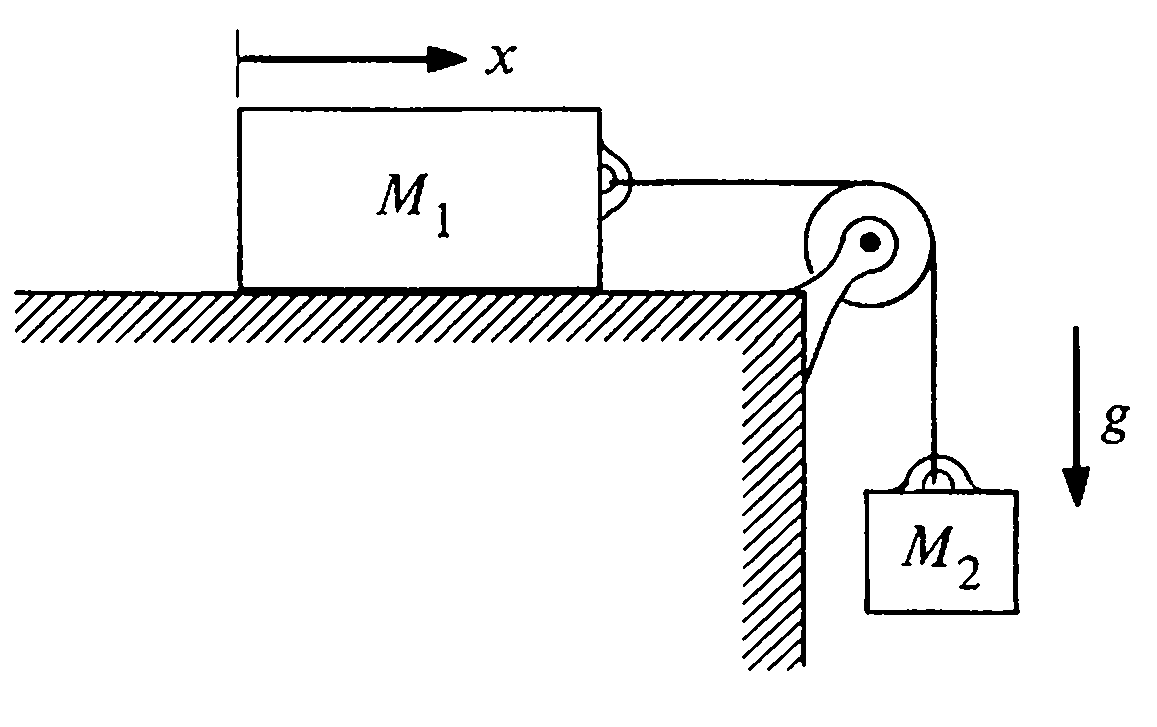
\includegraphics[width=0.35\textwidth]{ps02_1}\end{center}
\subsection{Solution}
  The system can be treated as a single block of mass $m_1 + m_2$, with a force due to gravity of $m_2 g$.  The acceleration is then $\frac{m_2 g}{m_1 + m_2}$, so the distance is $\frac{m_2 g}{2(m_1 + m_2)} t^2$.

  \noindent In more detail:
  \begin{center}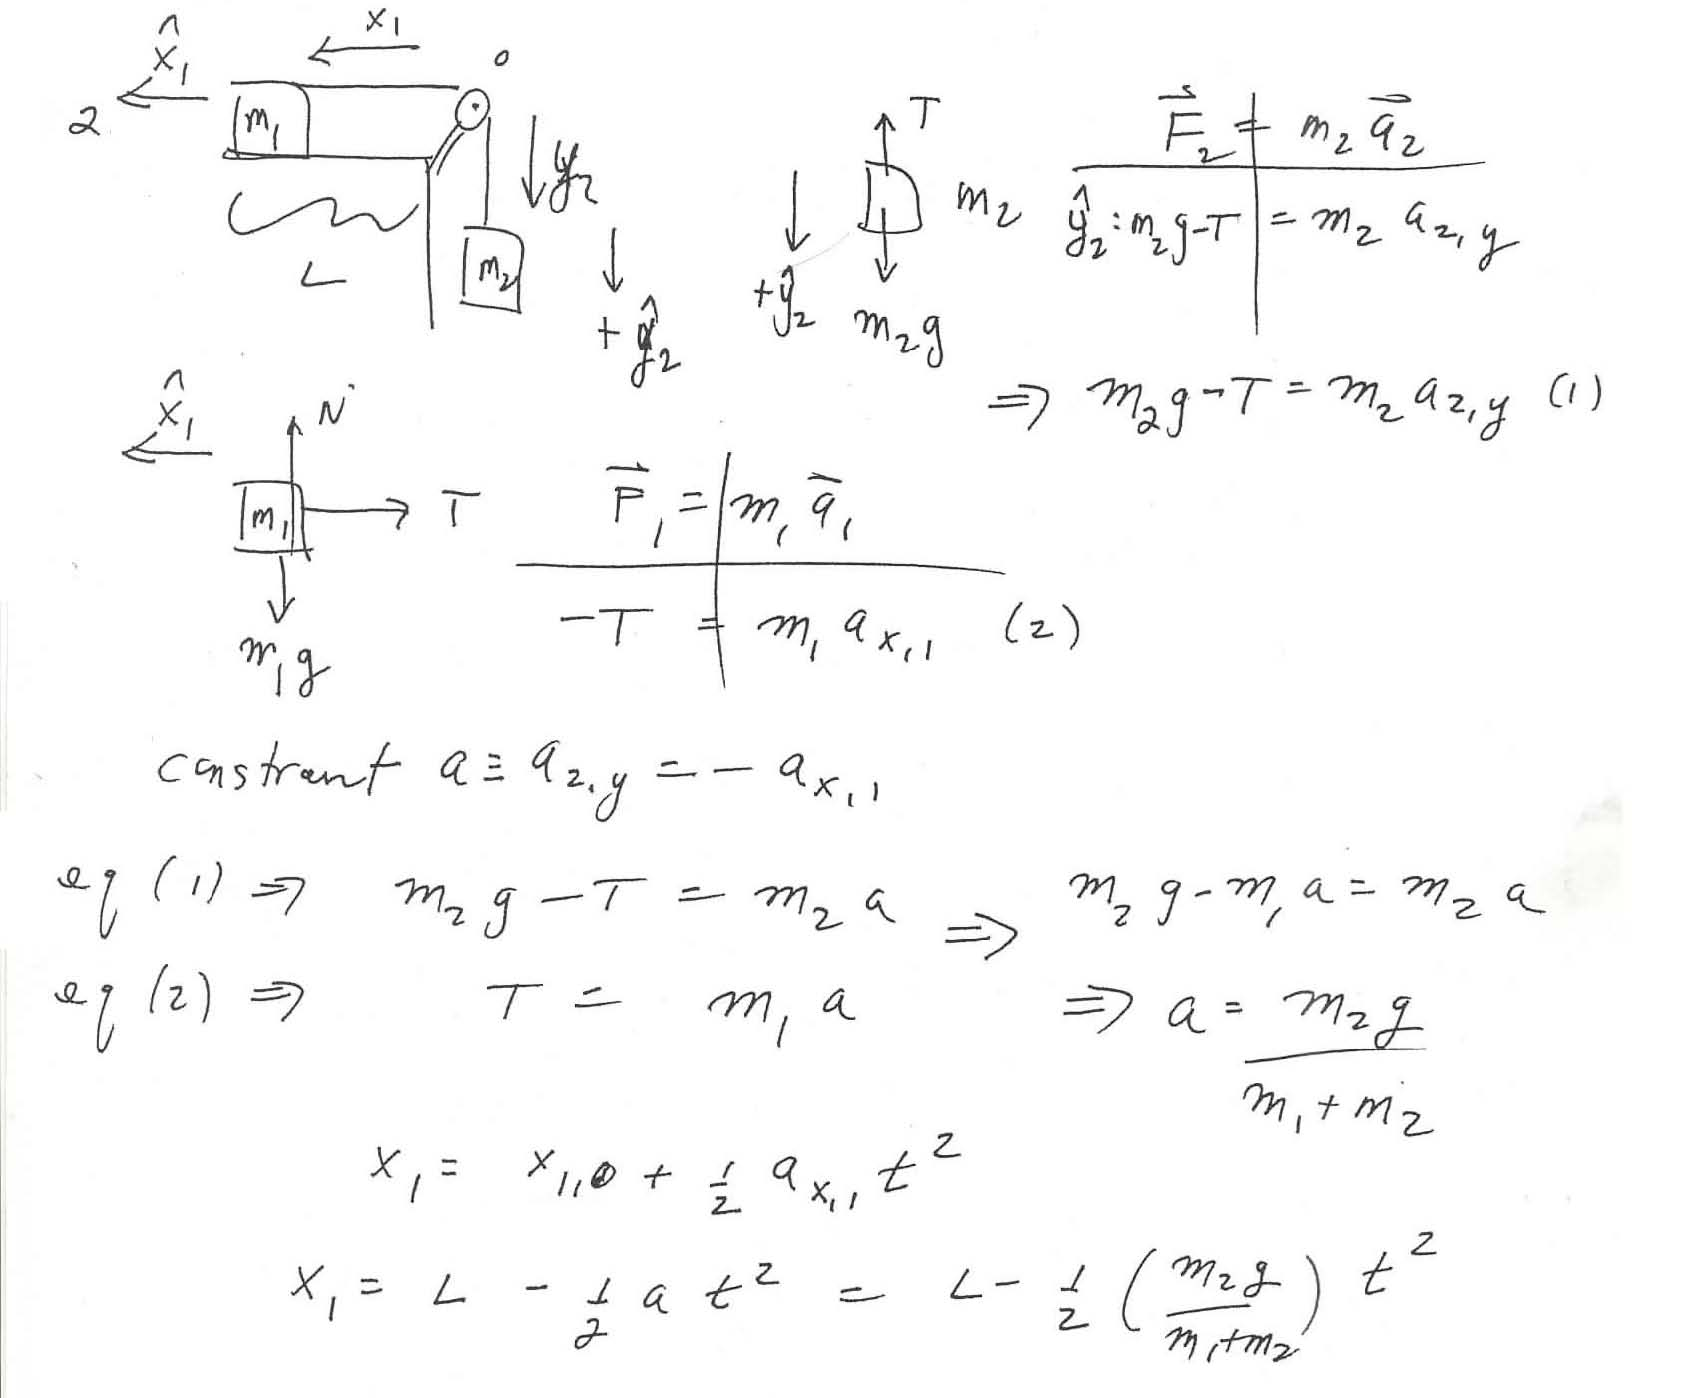
\includegraphics[width=\textwidth]{ps02_Solution_Problem_1}\end{center}
\section{Problem \thesection: K\&K 2.4}
\subsection{Problem}
  Two particles of mass $m_1$ and $m_2$ undergo uniform circular motion about each other at a separation $R$ under the influence of an attractive force of magnitude $F$.  The angular velocity is $\omega$ radians per second.
  \begin{enumerate}[a)]
    \item Show that $R = \frac{F}{\omega^2} \cdot \left(\frac{1}{m_1} + \frac{1}{m_2}\right)$.
    \item Explain why you can think of this problem as equivalent to a single body of mass $\mu$ where $\frac{1}{\mu} = \left(\frac{1}{m_1} + \frac{1}{m_2}\right)$ undergoing circular motion of radius $R$ due to the influence of a central attractive force of magnitude $F$.
  \end{enumerate}
\subsection{Solution}
  \begin{enumerate}[a)]
    \item Let $r_1$ and $r_2$ denote the radii of the circles of $m_1$ and $m_2$, respectively.  Then $R = r_1 + r_2$.  Since the movement is uniform and circular, the force must be $\frac{m_1 v_1^2}{r_1} = \frac{m_2 v_2^2}{r_2}$.  The acceleration of $m_1$ is then $\frac{v_1^2}{r_1}$, and the acceleration of $m_2$ is $\frac{v_2^2}{r_2}$.  Since the angular velocity is $\omega$, and the circumference is $2\pi r_1$ and $2\pi r_2$, respectively, $v_1 = \frac{2\pi r_1}{\frac{2\pi}{\omega}} = r_1 \omega$ and $v_2 = r_2 \omega$.  Then $F = m_1 r_1 \omega^2 =  m_2 r_2 \omega^2$.  Since $R = r_1 + r_2$, $F = m_1 r_1 \omega^2 = m_2 (R - r_1) \omega^2$.  So $F = m_1 r_1 \omega^2 = m_2 R \omega^2 - m_2 r_1 \omega^2$.  Dropping the $F$, $m_1 r_1 = m_2 R - m_2 r_1$, so $(m_1 + m_2)r_1 = m_2 R$.  Then $r_1 = \frac{R m_2}{m_1 + m_2}$.  Thus, $F =  \frac{R m_1 m_2\omega^2}{m_1 + m_2}$, so $R = \frac{F(m_1+m_2)}{\omega^2 m_1 m_2} = \frac{F}{\omega^2}\left(\frac{1}{m_1}+\frac{1}{m_2}\right)$.
    \item Let $\vec r_{AB} = \vec r_B - \vec r_A$ as shown below.
      \begin{center}
        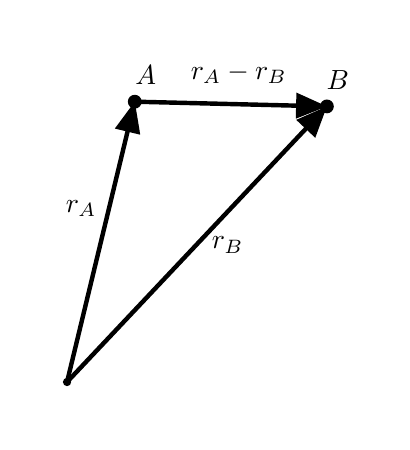
\begin{tikzpicture}[line cap=round,line join=round,>=triangle 45,x=1.0cm,y=1.0cm]
        \clip(-0.5,-0.5) rectangle (4,4.5);
        \draw [->,line width=1.6pt] (0.86,3.56) -- (3.3,3.5);
        \draw [->,line width=1.6pt] (0,0) -- (0.86,3.56);
        \draw [->,line width=1.6pt] (0,0) -- (3.3,3.5);
        \fill [color=black] (0,0) circle (1.5pt);
        \fill [color=black] (0.86,3.56) circle (2.5pt);
        \draw[color=black] (1,3.9) node {$A$};
        \fill [color=black] (3.3,3.5) circle (2.5pt);
        \draw[color=black] (3.44,3.84) node {$B$};
        \draw[color=black] (2.18,3.92) node {$r_A - r_B$};
        \draw[color=black] (0.18,2.2) node {$r_A$};
        \draw[color=black] (2.04,1.74) node {$r_B$};
        \end{tikzpicture}
      \end{center}
      Then $\vec F_{AB} = m_B \vec a_B$ and $\vec F_{BA} = m_A \vec a_A = -\vec F_{AB}$.  $\frac{\vec F_{AB}}{m_B} - \frac{\vec F_{BA}}{m_A} = \vec a_B - \vec a_A$, so $\vec F_{AB}\left(\frac{1}{m_A} + \frac{1}{m_B}\right) = \frac{\partial^2}{\partial t^2}(\vec r_B - \vec r_A)$.  Then $\vec F_{AB}\left(\frac{1}{m_A} + \frac{1}{m_B}\right) = \frac{\partial^2}{\partial t^2}\vec r_{AB}$.  Define $\mu$ such that $\frac{1}{\mu} = \frac{1}{m_A} + \frac{1}{m_B}$, and $\omega$ to be $\left\vert \frac{\partial \hat r_{AB}}{\partial t}\right\vert$.  Then $\vec F_{AB} = \mu \frac{\partial^2}{\partial t^2}\vec r_{AB} = -\mu R\omega^2\hat r_{AB}$, since the vector is rotating with uniform angular momentum.  Then $R = \frac{F}{\omega^2}\mu$, which corresponds to the setup in (a).
  \end{enumerate}

  \noindent With diagrams:
  \begin{center}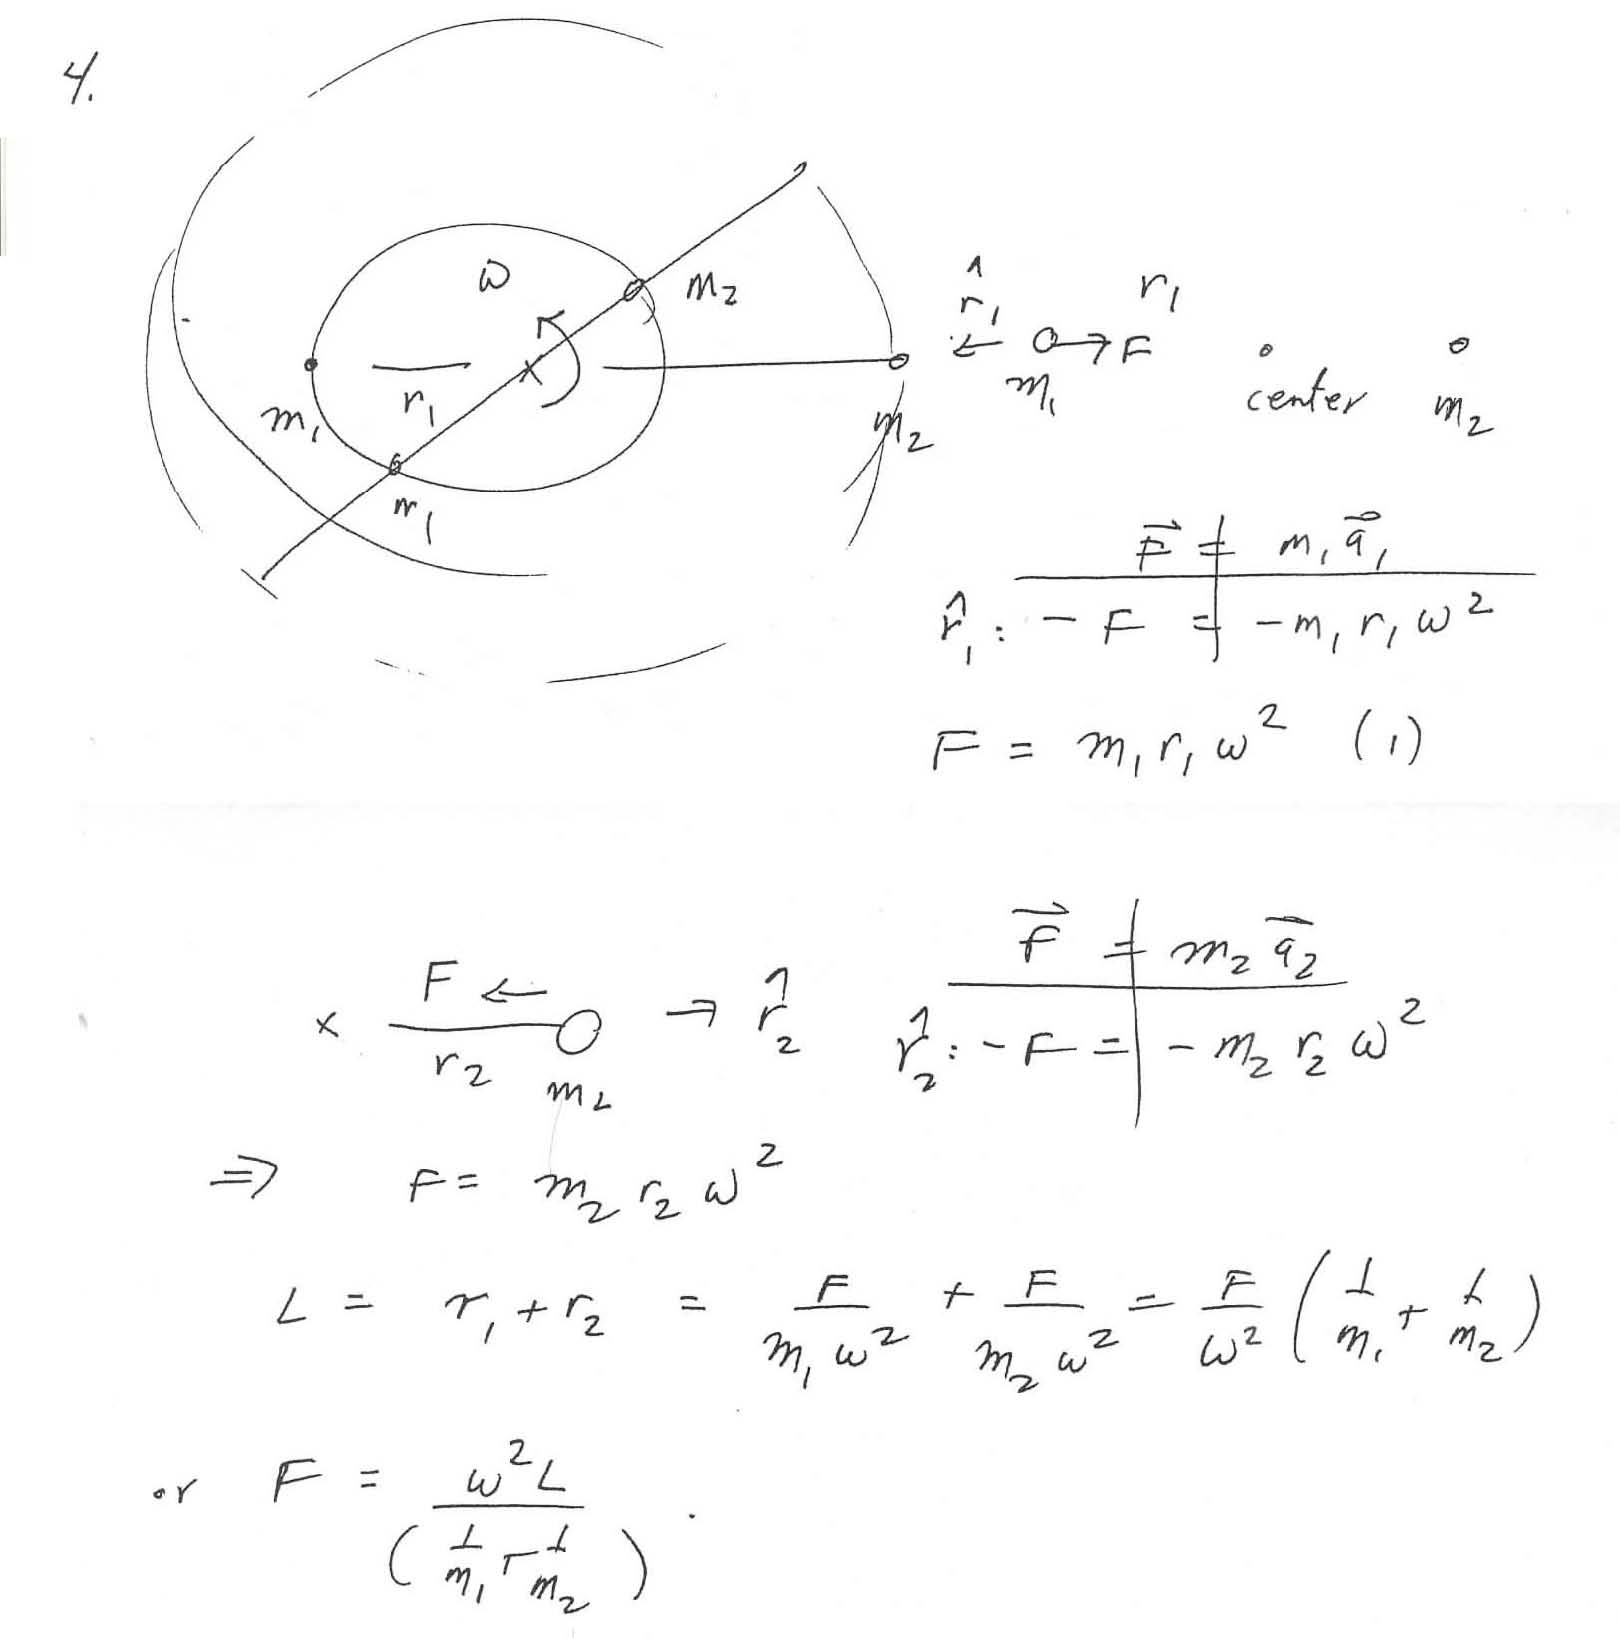
\includegraphics[width=\textwidth]{ps02_Solution_Problem_2}\end{center}
\section{Problem \thesection: K\&K 2.7}
\subsection{Problem}
  Consider two textbooks that are resting one on top of the other. The lower book has $m_2 = 0.8$ kg and is resting on a nearly frictionless surface. The upper book has mass $m_1 = 2.0$ kg. Suppose the coefficient of static friction is given by $\mu_s = 0.1$.
  \begin{center}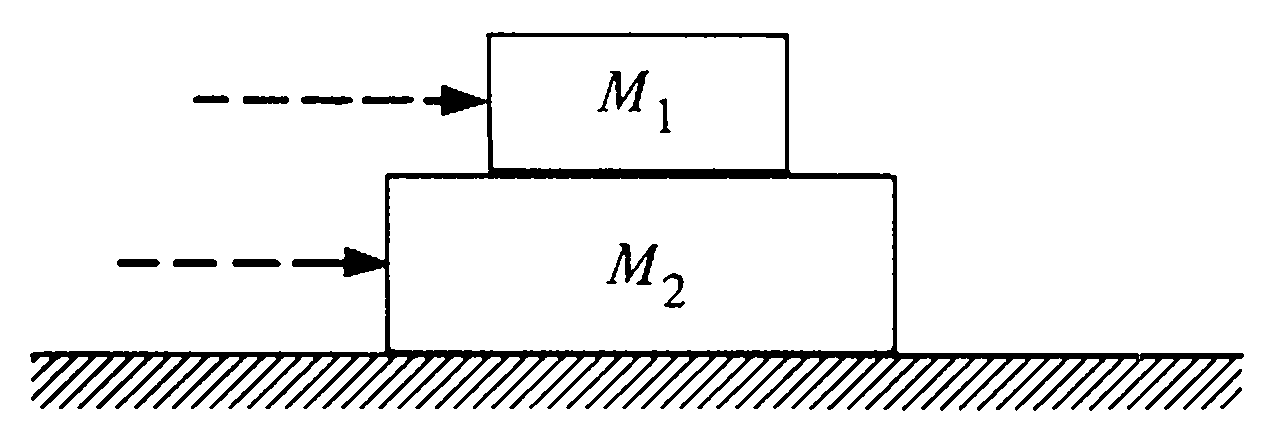
\includegraphics[width=0.35\textwidth]{ps02_2}\end{center}
  \begin{enumerate}[a)]
    \item What is the maximum force which the upper book can be pushed horizontally so that the two books move together without slipping? Identify all action-reaction pairs of forces in this problem.
    \item What is the maximum force which the lower book can be pushed horizontally so that the two books move together without slipping? Identify all action-reaction pairs of forces in this problem.
    \item Explain why one of your forces in parts a) and b) is larger than the other.
  \end{enumerate}
\subsection{Solution}
  \begin{enumerate}[a)]
    \item The top block exerts friction on the bottom block, and vice versa.  Gravity exerts a force on each block, and the surface below exerts a normal force.  The blocks can be treated as a single block with mass $m_1 + m_2$ to which $F_{\text{applied}}$ is applied.  The acceleration is $\frac{F_{\text{applied}}}{m_1 + m_2}$.  The maximal force due to friction is $\mu_s F_n = m_1 g \mu_s$.  The maximal acceleration of the top block is thus $\frac{\mu_s m_1 g}{m_1} = \mu_s g = 1$ m / s$^2$.  Thus, the maximal applied force is $(1\text{ m / s}^2)(m_1 + m_2) = 3$ N.
      \begin{center}
        \definecolor{uququq}{rgb}{0.25,0.25,0.25}
        \begin{tikzpicture}[line cap=round,line join=round,>=triangle 45,x=1.0cm,y=1.0cm]
        \clip(0.75,-0.25) rectangle (2.25,1);
        \fill[fill=black,fill opacity=0.25] (0,0) -- (3.48,0) -- (6.46,-2.52) -- (-2.74,-2.68) -- cycle;
        \fill[fill=black,fill opacity=0.05] (0.93,0.35) -- (2.17,0.35) -- (2.17,0) -- (0.93,0) -- cycle;
        \fill[fill=black,fill opacity=0.05] (1.14,0.62) -- (1.96,0.62) -- (1.96,0.35) -- (1.14,0.35) -- cycle;
        \draw (0,0)-- (3.48,0);
        \draw (3.48,0)-- (6.46,-2.52);
        \draw (6.46,-2.52)-- (-2.74,-2.68);
        \draw (-2.74,-2.68)-- (0,0);
        \draw (0.93,0.35)-- (2.17,0.35);
        \draw (2.17,0.35)-- (2.17,0);
        \draw (2.17,0)-- (0.93,0);
        \draw (0.93,0)-- (0.93,0.35);
        \draw (1.14,0.62)-- (1.96,0.62);
        \draw (1.96,0.62)-- (1.96,0.35);
        \draw (1.96,0.35)-- (1.14,0.35);
        \draw (1.14,0.35)-- (1.14,0.62);
        \draw [->,line width=1.6pt] (1.55,0.49) -- (1.55,0.77);
        \draw [->,line width=1.6pt] (1.55,0.49) -- (1.55,0.2);
        \draw [->,line width=1.6pt] (1.55,0.18) -- (2.06,0.18);
        \draw [->,line width=1.6pt] (1.55,0.49) -- (2.17,0.49);
        \draw [->,line width=1.6pt] (1.55,0.49) -- (1.04,0.49);
        \draw[color=black] (1.57,0.15) node {$M_2$};
        \draw[color=black] (1.52,0.54) node {$M_1$};
        \fill [color=uququq] (1.55,0.49) circle (1.5pt);
        \fill [color=uququq] (1.55,0.18) circle (1.5pt);
        \draw[color=black] (1.57,0.82) node {$F_N$};
        \draw[color=black] (1.51,0.26) node {$F_g$};
        \draw[color=black] (2.11,0.16) node {$F_\text{fr}$};
        \draw[color=black] (2.11,0.45) node {$F_\text{applied}$};
        \draw[color=black] (1.09,0.46) node {$F_\text{fr}$};
        \end{tikzpicture} % Diagram 2
      \end{center}
    \item The top block exerts friction on the bottom block, and vice versa.  Gravity exerts a force on each block, and the surface below exerts a normal force.  The blocks can be treated as a single block with mass $m_1 + m_2$ to which $F_{\text{applied}}$ is applied.  The acceleration is $\frac{F_{\text{applied}}}{m_1 + m_2}$.  The maximal force due to friction is $\mu_s F_n = m_1 g \mu_s$.  The maximal acceleration of the top block is thus $\frac{\mu_s m_1 g}{m_2} = 2.45\text{ m / s}^2\approx 2$ m / s$^2$.  Thus, the maximal applied force is $(2\text{ m / s}^2)(m_1 + m_2) = 7$ N.
      \begin{center}
        \definecolor{uququq}{rgb}{0.25,0.25,0.25}
        \begin{tikzpicture}[line cap=round,line join=round,>=triangle 45,x=1.0cm,y=1.0cm]
        \clip(0.75,-0.25) rectangle (2.5,1);
        \fill[fill=black,fill opacity=0.25] (0,0) -- (3.48,0) -- (6.46,-2.52) -- (-2.74,-2.68) -- cycle;
        \fill[fill=black,fill opacity=0.05] (0.93,0.35) -- (2.17,0.35) -- (2.17,0) -- (0.93,0) -- cycle;
        \fill[fill=black,fill opacity=0.05] (1.14,0.62) -- (1.96,0.62) -- (1.96,0.35) -- (1.14,0.35) -- cycle;
        \draw (0,0)-- (3.48,0);
        \draw (3.48,0)-- (6.46,-2.52);
        \draw (6.46,-2.52)-- (-2.74,-2.68);
        \draw (-2.74,-2.68)-- (0,0);
        \draw (0.93,0.35)-- (2.17,0.35);
        \draw (2.17,0.35)-- (2.17,0);
        \draw (2.17,0)-- (0.93,0);
        \draw (0.93,0)-- (0.93,0.35);
        \draw (1.14,0.62)-- (1.96,0.62);
        \draw (1.96,0.62)-- (1.96,0.35);
        \draw (1.96,0.35)-- (1.14,0.35);
        \draw (1.14,0.35)-- (1.14,0.62);
        \draw [->,line width=1.6pt] (1.55,0.49) -- (2.09,0.49);
        \draw [->,line width=1.6pt] (1.55,0.49) -- (1.55,0.7);
        \draw [->,line width=1.6pt] (1.55,0.49) -- (1.55,0.27);
        \draw [->,line width=1.6pt] (1.55,0.18) -- (2.35,0.18);
        \draw [->,line width=1.6pt] (1.55,0.18) -- (1.01,0.18);
        \draw[color=black] (1.57,0.15) node {$M_2$};
        \draw[color=black] (1.5,0.5) node {$M_1$};
        \fill [color=uququq] (1.55,0.49) circle (1.5pt);
        \fill [color=uququq] (1.55,0.18) circle (1.5pt);
        \draw[color=black] (2.11,0.56) node {$F_\text{fr}$};
        \draw[color=black] (1.57,0.79) node {$F_N$};
        \draw[color=black] (1.61,0.27) node {$F_g$};
        \draw[color=black] (2.29,0.15) node {$F_\text{applied}$};
        \draw[color=black] (1.07,0.24) node {$F_\text{fr}$};
        \end{tikzpicture}
      \end{center}  % Diagram 1
    \item The maximal acceleration due to friction is the same in both cases, but the acceleration is of a larger mass in part b), so more force can be applied.
  \end{enumerate}

  \noindent In more detail:
  \begin{center}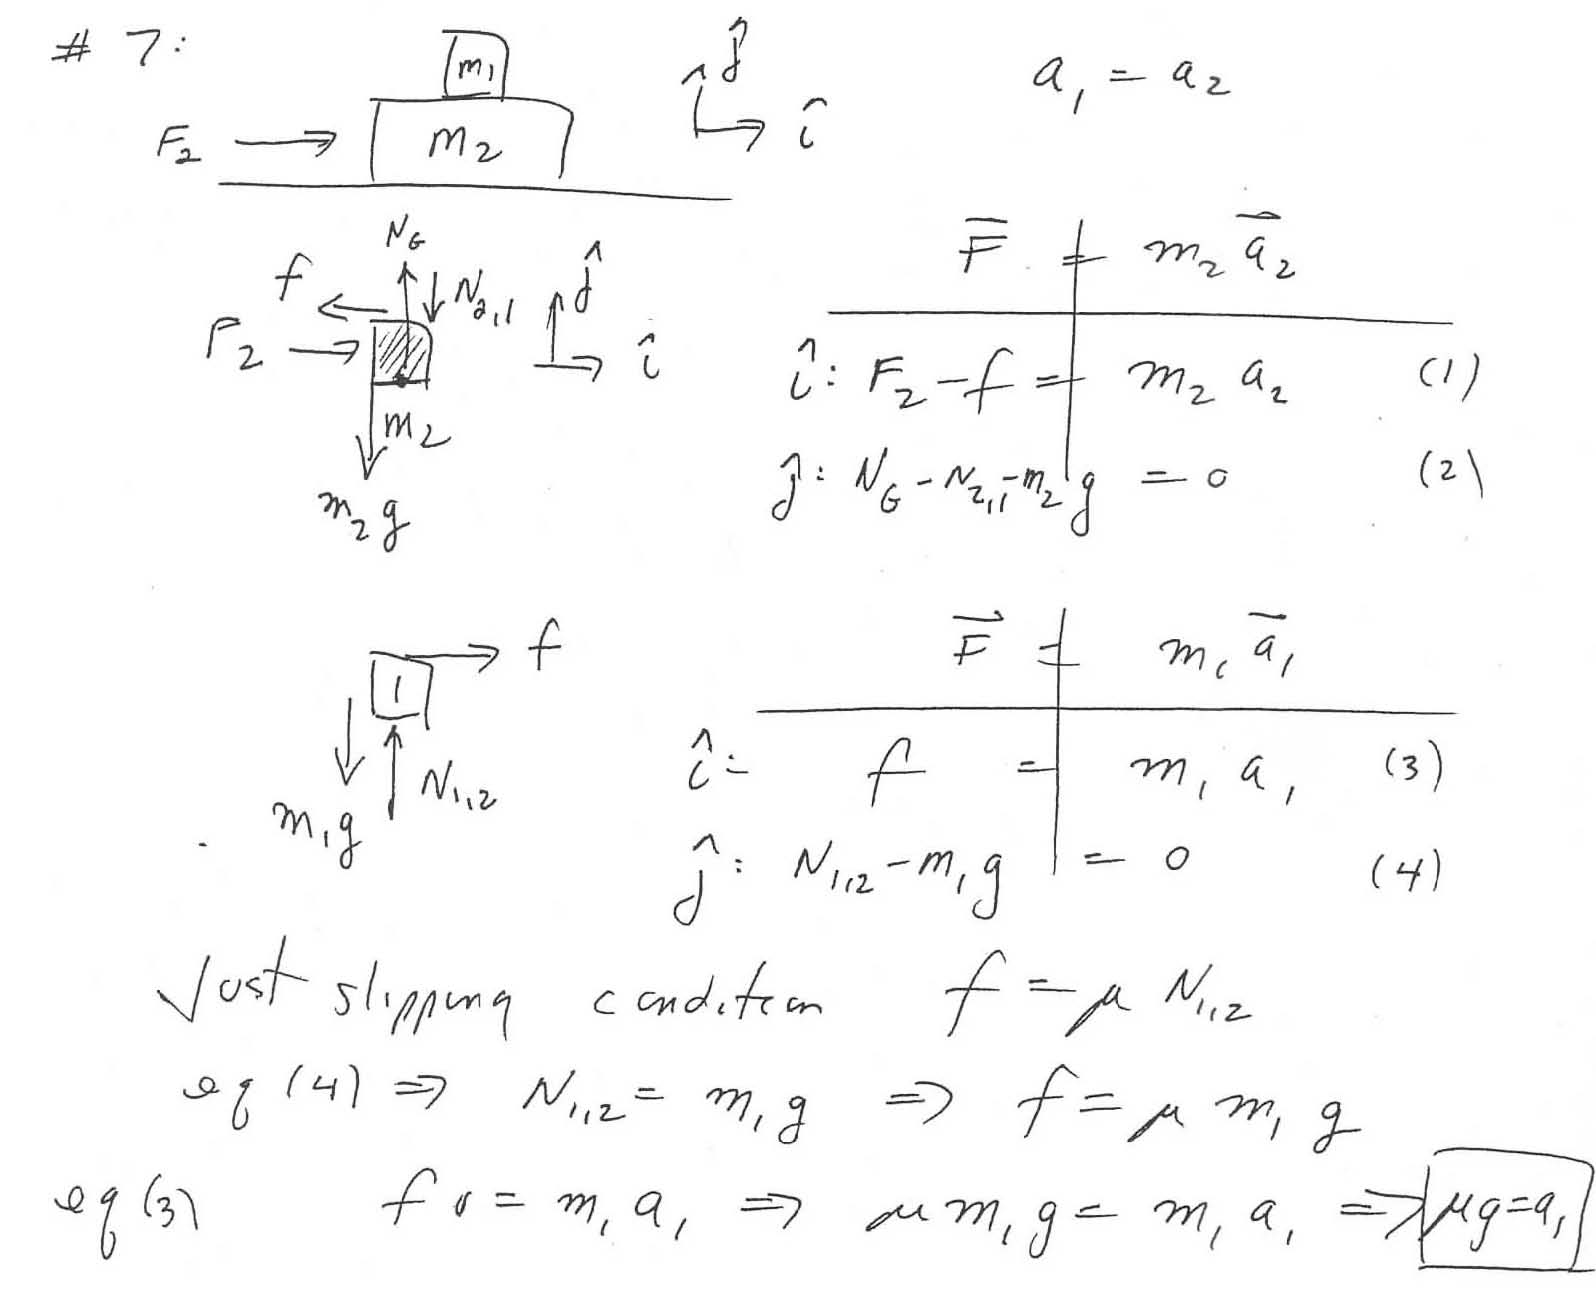
\includegraphics[width=\textwidth]{ps02_Solution_Problem_3_0}\end{center}
  \begin{center}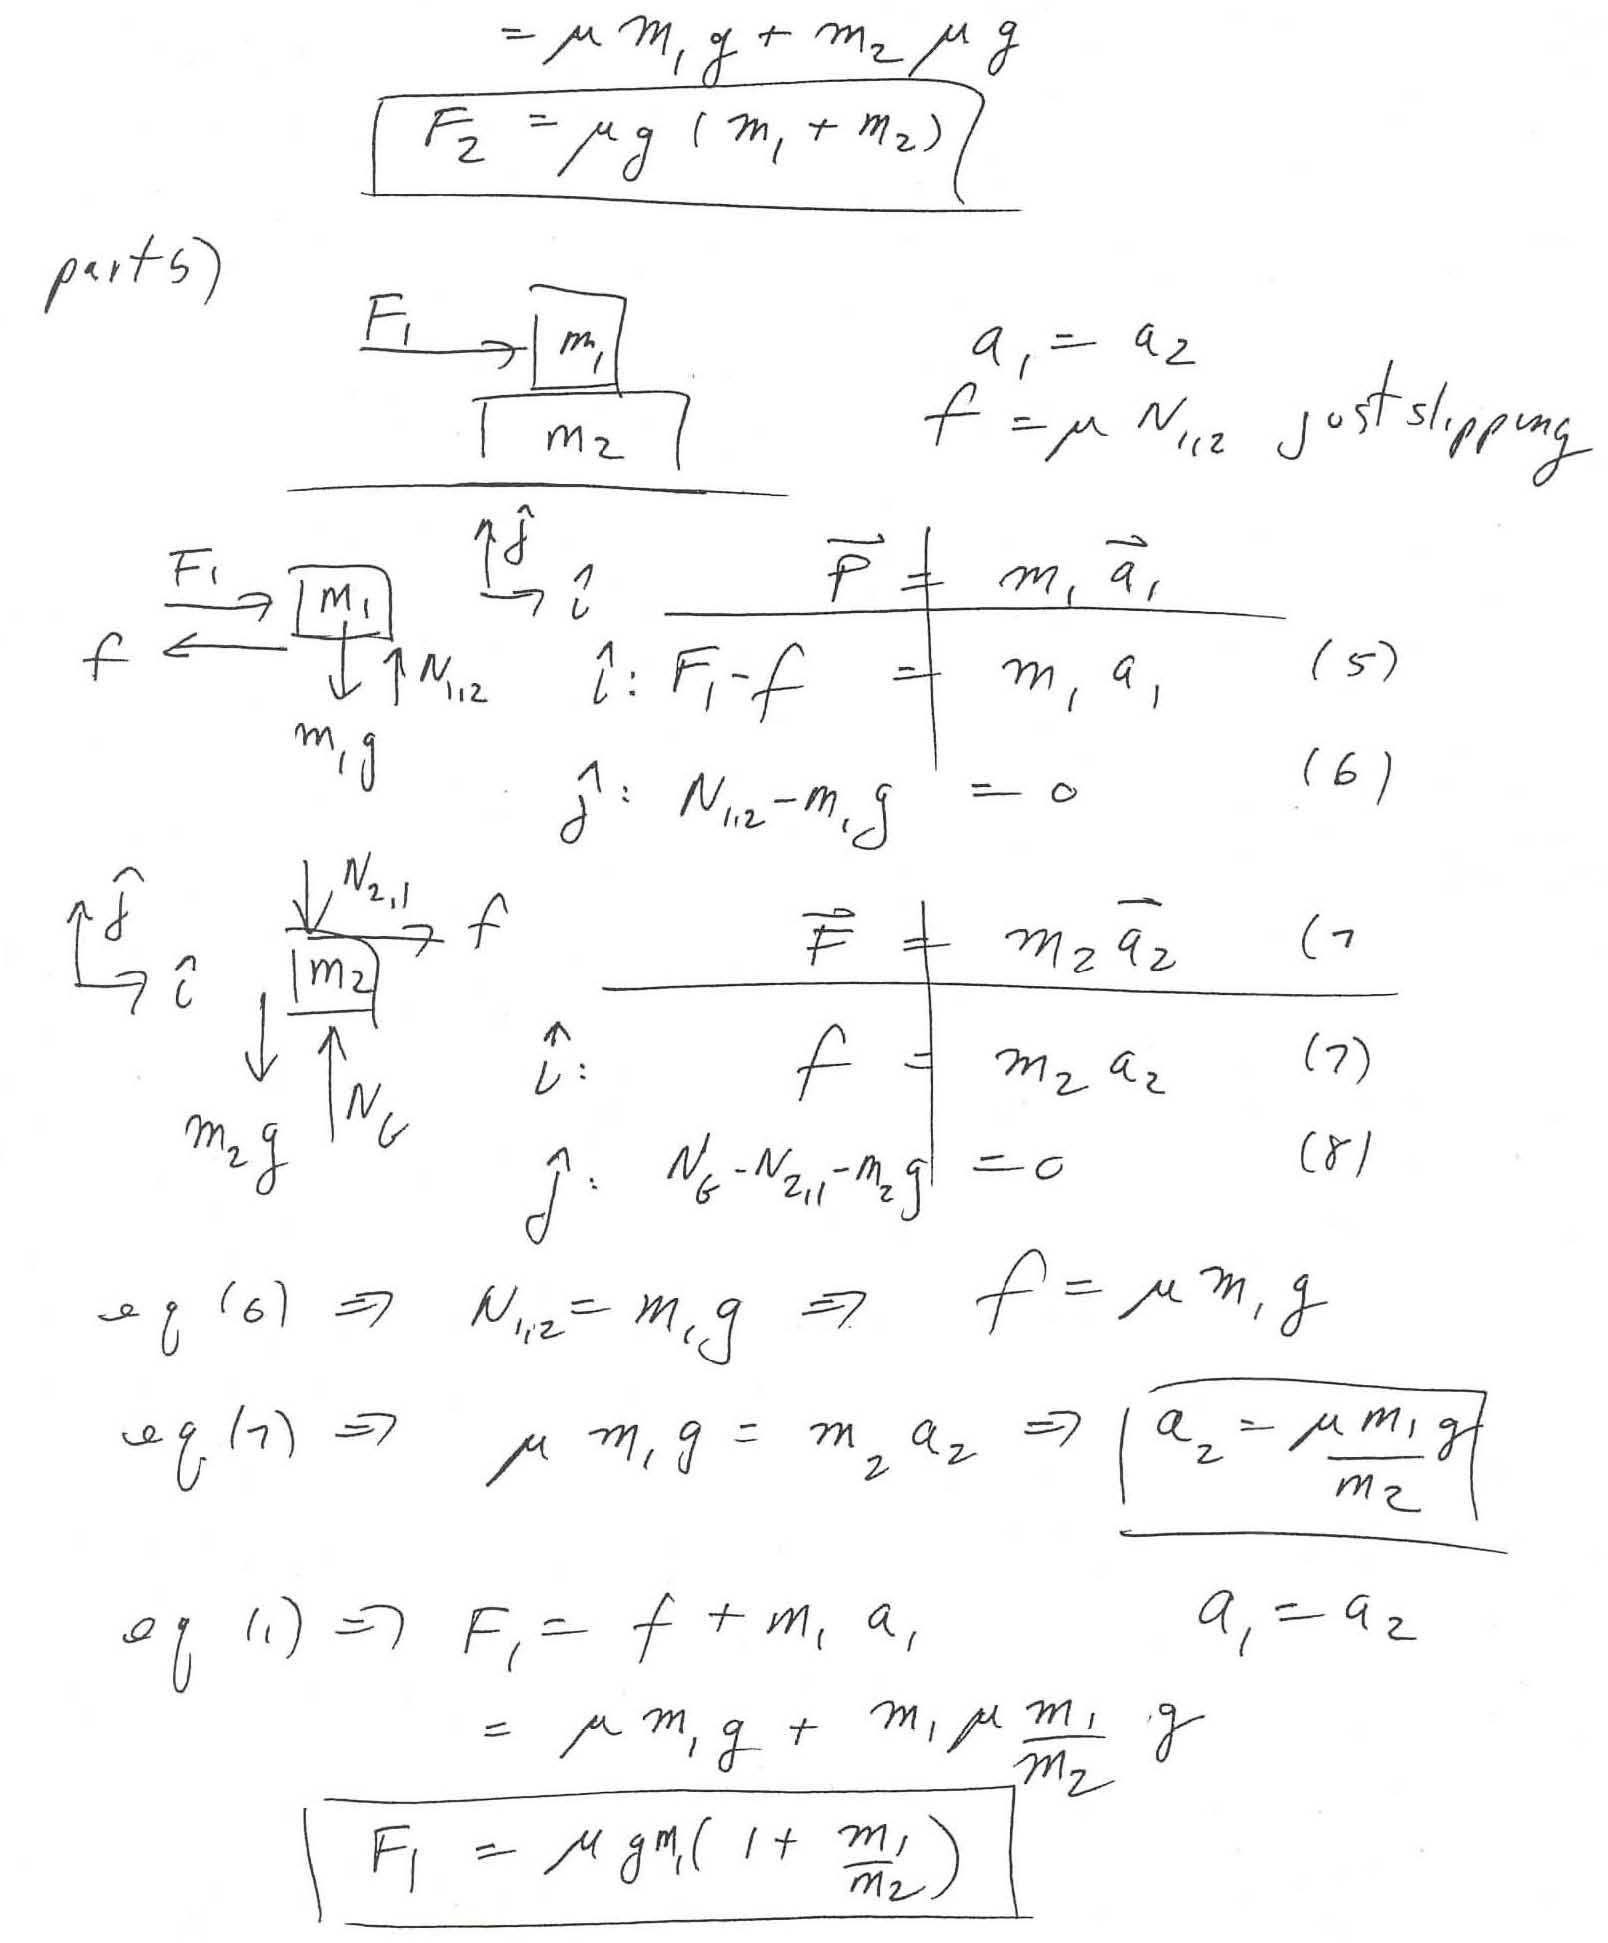
\includegraphics[width=\textwidth]{ps02_Solution_Problem_3_1}\end{center}
\section{Problem \thesection: K\&K 2.9}
\subsection{Problem}
  A body of mass $m$ is moving in a horizontal circle of radius $r$ with a constant speed $v_0$ on the inside wall of a cone. Assume the wall of the cone is frictionless. The wall of the cone makes an angle $\theta$ with the vertical.
  \begin{center}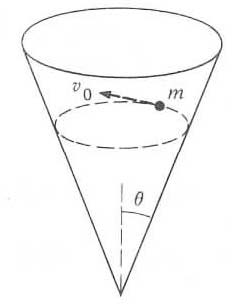
\includegraphics[width=0.2\textwidth]{ps02_3}\end{center}
  \begin{enumerate}[a)]
    \item Draw a free body force diagram showing all the forces acting on the mass.
    \item What is the speed, $v_0$, of the body, in terms of $r$, $m$, $\theta$, and $g$?
    \item How long will the mass take to go around the circle?
    \item Now assume there is a coefficient of static friction $\mu_s$. Find the maximum speed the mass can move on the inside of a cone and still move in a circular orbit of radius $r$.
  \end{enumerate}
\subsection{Solution}
  \begin{enumerate}[a)]
    \item $\left.\right.$\par\noindent
      \begin{center}
        \definecolor{uququq}{rgb}{0.25,0.25,0.25}
        \begin{tikzpicture}[line cap=round,line join=round,>=triangle 45,x=1.0cm,y=1.0cm]
        \clip(-0.25,-0.25) rectangle (3.5,5);
        \draw [shift={(0,0)},fill=black,fill opacity=0.1] (0,0) -- (51.58:0.37) arc (51.58:90:0.37) -- cycle;
        \fill[fill=black,fill opacity=0.1] (2.66,3.35) -- (2.17,3.74) -- (1.4,2.76) -- (1.88,2.38) -- cycle;
        \draw (2.66,3.35)-- (2.17,3.74);
        \draw (2.17,3.74)-- (1.4,2.76);
        \draw (1.4,2.76)-- (1.88,2.38);
        \draw (1.88,2.38)-- (2.66,3.35);
        \draw [->,line width=1.6pt] (2.03,3.06) -- (0.49,4.28);
        \draw [->,line width=1.6pt] (2.03,3.06) -- (2.03,1.83);
        \draw (0,0)-- (3.35,4.23);
        \draw [dash pattern=on 3pt off 3pt] (0,4.23)-- (0,0);
        \draw[color=black] (0.33,0.49) node {$\theta$};
        \fill [color=uququq] (2.03,3.06) circle (1.5pt);
        \draw[color=black] (0.68,4.48) node {$F_N$};
        \draw[color=black] (2.23,1.87) node {$F_g$};
        \end{tikzpicture}
      \end{center} % diagram 3
    \item For circular motion, $\frac{\partial \vec r}{\partial t} = r\frac{\partial \theta}{\partial t}\hat \theta = v_0 \hat \theta$, so $\frac{\partial^2 \vec r}{\partial t^2} = -r\left(\frac{\partial \theta}{\partial t}\right)^2\hat r = -\frac{v_0^2}{r}\hat r$.  Since $F_N\sin\theta = mg$, and $\vec F_{\text{net}} = -F_N\cos\theta\hat i$, $\frac{mg}{\sin\theta}\cos\theta = m\frac{v_0^2}{r}$, so $v_0 = \sqrt{gr\cot\theta}$.
    \item The circumference is $2\pi r$, and $v_0 = \sqrt{gr\cot\theta}$, so it takes $\frac{2\pi\sqrt{r}}{\sqrt{g\cot\theta}}$.
    \item FIX The diagram becomes: \begin{center}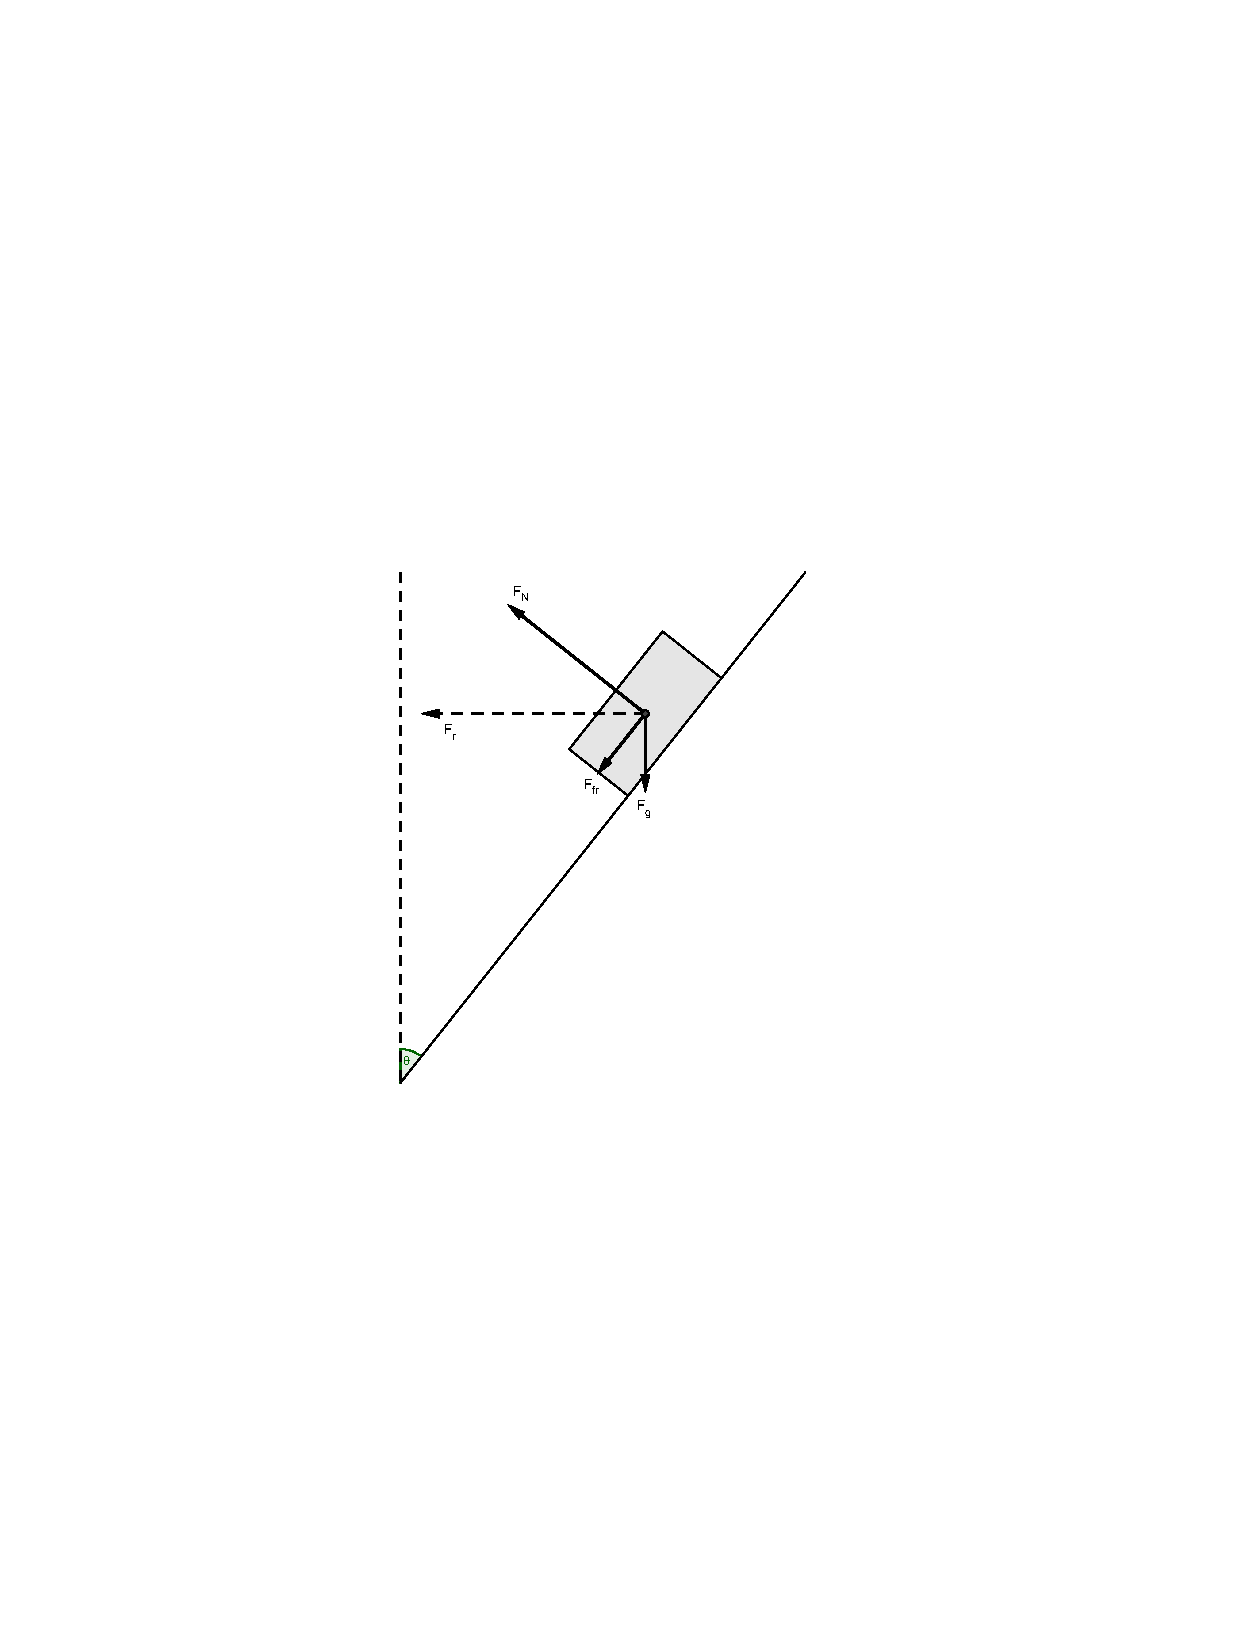
\includegraphics[width=0.25\textwidth]{2009-09-25_Diagram_8}\end{center}  Decomposing the vectors, \begin{center}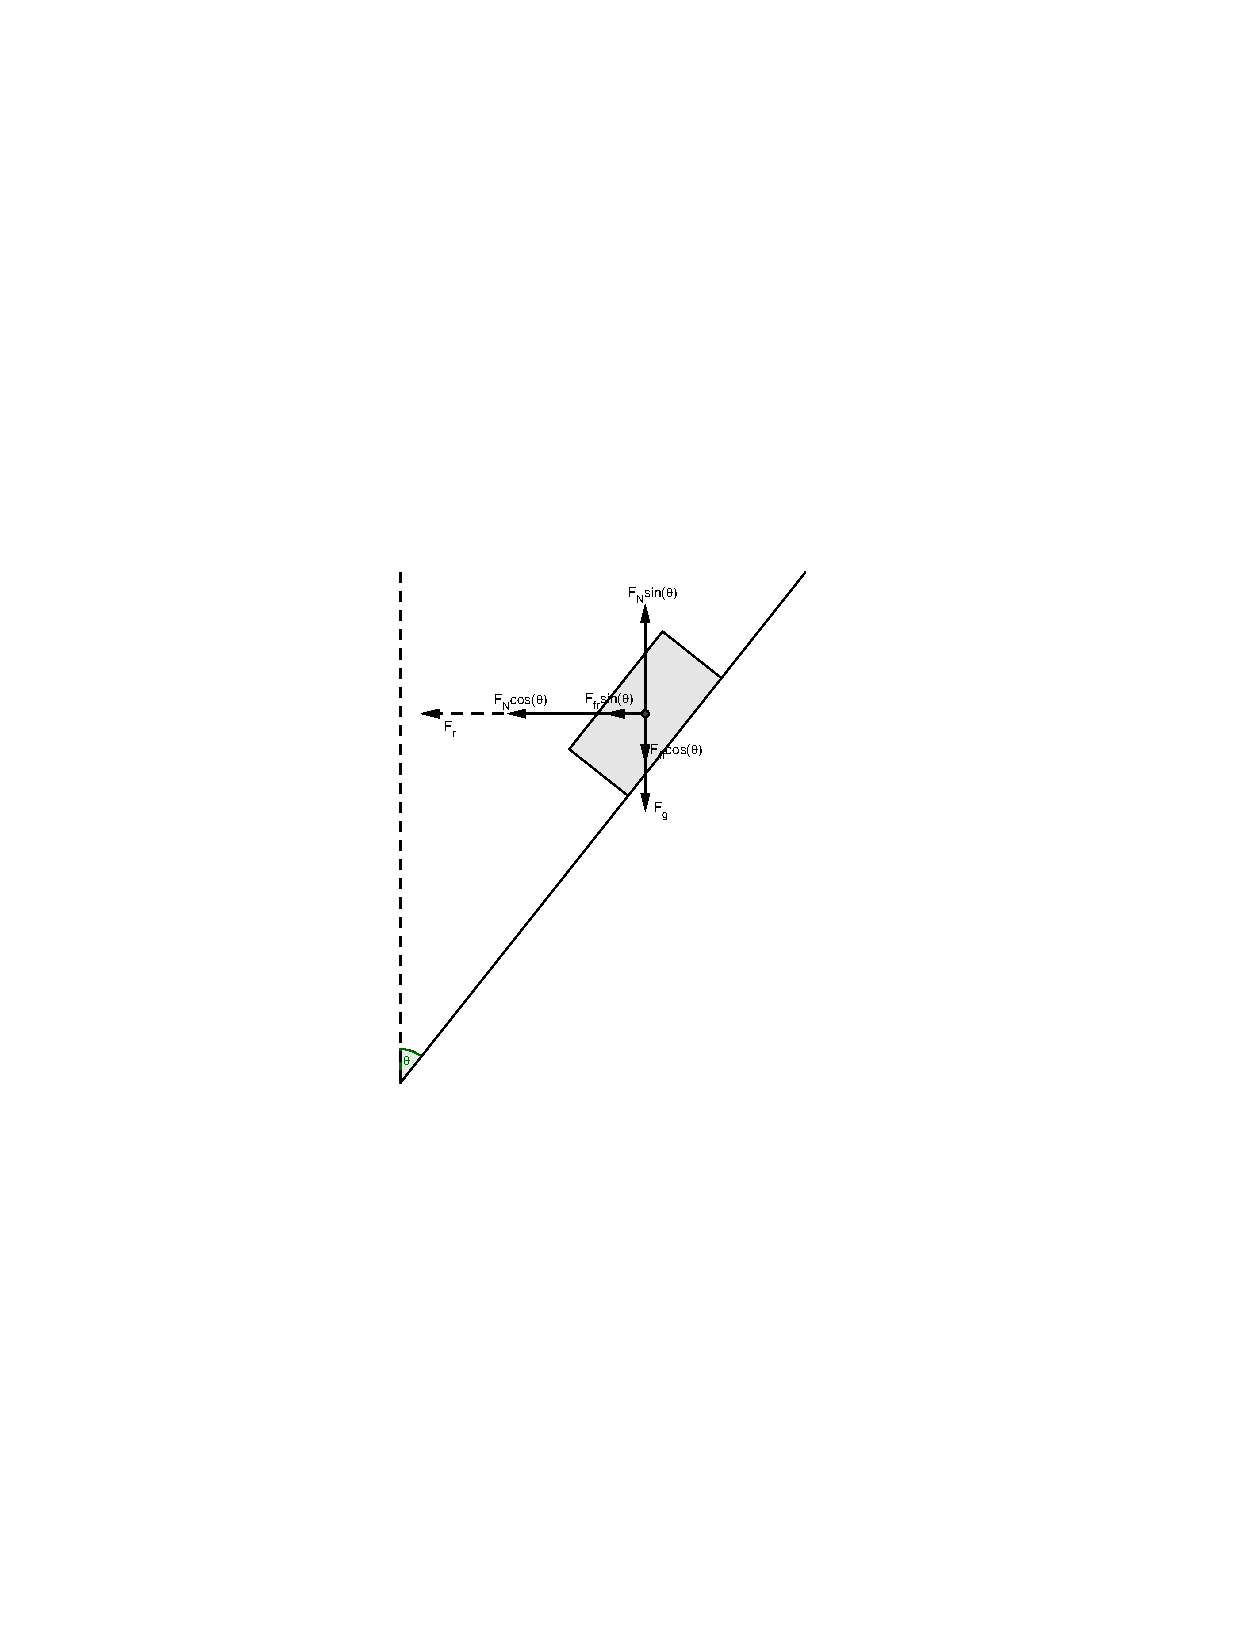
\includegraphics[width=0.25\textwidth]{2009-09-25_Diagram_9}\end{center}  The radial acceleration is $\frac{v^2}{r}$, so $\frac{\partial^2 \vec r}{\partial t^2} = -\frac{v^2}{r}\hat i$.  Then $m\frac{v^2}{r} = F_{\text{fr}}\sin\theta + F_g\cos\theta = F_N \mu_s + F_g\cos\theta$.  The normal force is $m\frac{v^2}{r}\cos\theta$.  Then $m\frac{v^2}{r} = m\frac{v^2}{r}\cos\theta \mu_s + mg\cos\theta$, so $\frac{v^2}{r}(1 - \cos\theta \mu_s) = g\cos\theta$, so $v = \sqrt{\frac{rg\cos\theta}{1-\cos\theta\mu_s}}$. ???
  \end{enumerate}

  \noindent
\section{Problem \thesection: K\&K 2.10}
\subsection{Problem}
  The earth is spinning about its axis with a period of 23 hours 56 min and 4 sec. The equatorial radius of the earth is $6.38\cdot 10^{6}$ m. The latitude of Cambridge, Mass is 42$^{\circ}$ 22'.
  \begin{enumerate}[a)]
    \item Find the velocity of a person at MIT as they undergo circular motion about the earth? axis of rotation.
    \item Find the person's centripetal acceleration.
    \item The rotation of the Earth is slowing down. In 1977, the Earth took 1.01s longer to complete 365 rotations than in 1900. What was the average angular deceleration of the Earth in the time interval from 1900 to 1977?
    \item Find the radius of the orbit of a synchronous satellite which circles the earth. (A synchronous satellite goes around the earth once every rotation of the earth, so that its position appears stationary with respect to a ground station).  \par\noindent
      Note: You may need to use the fact that the force of gravity between two objects of masses $m_1$ and $m_2$, separated by a distance $d$, is $F_g = \frac{G m_1 m_2}{d^2}$, where $G$ is the universal constant of gravitation.
  \end{enumerate}
\subsection{Solution}
  \begin{enumerate}[a)]
    \item The radius of the circle of rotation is $r_E \cos(42^{\circ} 22') \approx 4710$ km.  The circumference is then about 29600 km.  The velocity is thus $\frac{29600\text{ km}}{23\text{ h }56\text{ m }4\text{ s}} \approx 343$ m/s.
    \item The centripetal acceleration is $\frac{v^2}{r} \approx 0.0251$ m / s$^2$.
    \item The angular velocity is $\frac{2\pi}{t}$, so the angular deceleration is $\frac{\frac{365\cdot 2\pi}{1\text{ year}} - \frac{365\cdot 2\pi}{1\text{ year}+1.01\text{ s}}}{77\text{ years}} \approx 10^{-21}$ s$^{-2}$.
    \item Since $v = \frac{2\pi r}{t}$, $a = G\frac{m_e}{r^2} = \frac{4\pi^2 r}{t^2}$, so $r = \sqrt[3]{\frac{G t^2}{4\pi^2}} \approx 42000$ km.
  \end{enumerate}
\section{Problem \thesection: K\&K 2.16}
\subsection{Problem}
  A 45$^{\circ}$ wedge is pushed along a table with constant acceleration $A$. A block of mass $m$ slides without friction down the wedge. Find its acceleration. (Gravity is directed down.)
  \begin{center}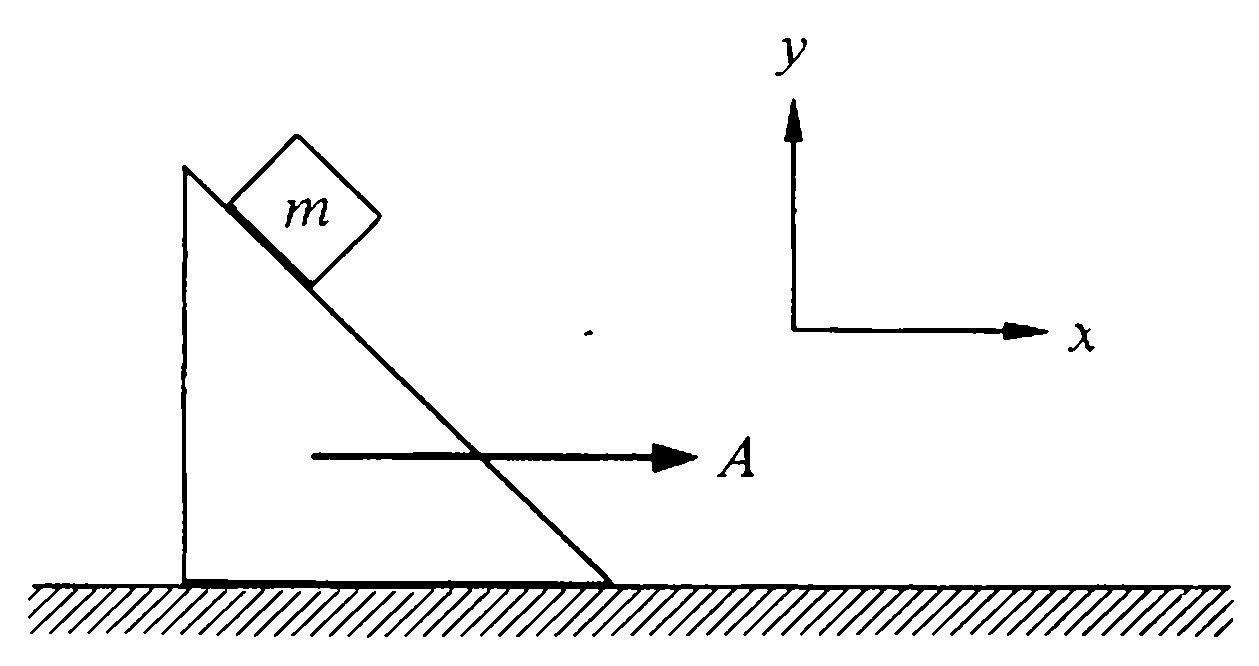
\includegraphics[width=0.35\textwidth]{ps02_4}\end{center}
\subsection{Solution}
  We begin with a coordinate transformation, substituting the acceleration of the wedge, $\vec A$, with a force in the opposite direction, $\vec F_A = -m \vec A$.
  \begin{center}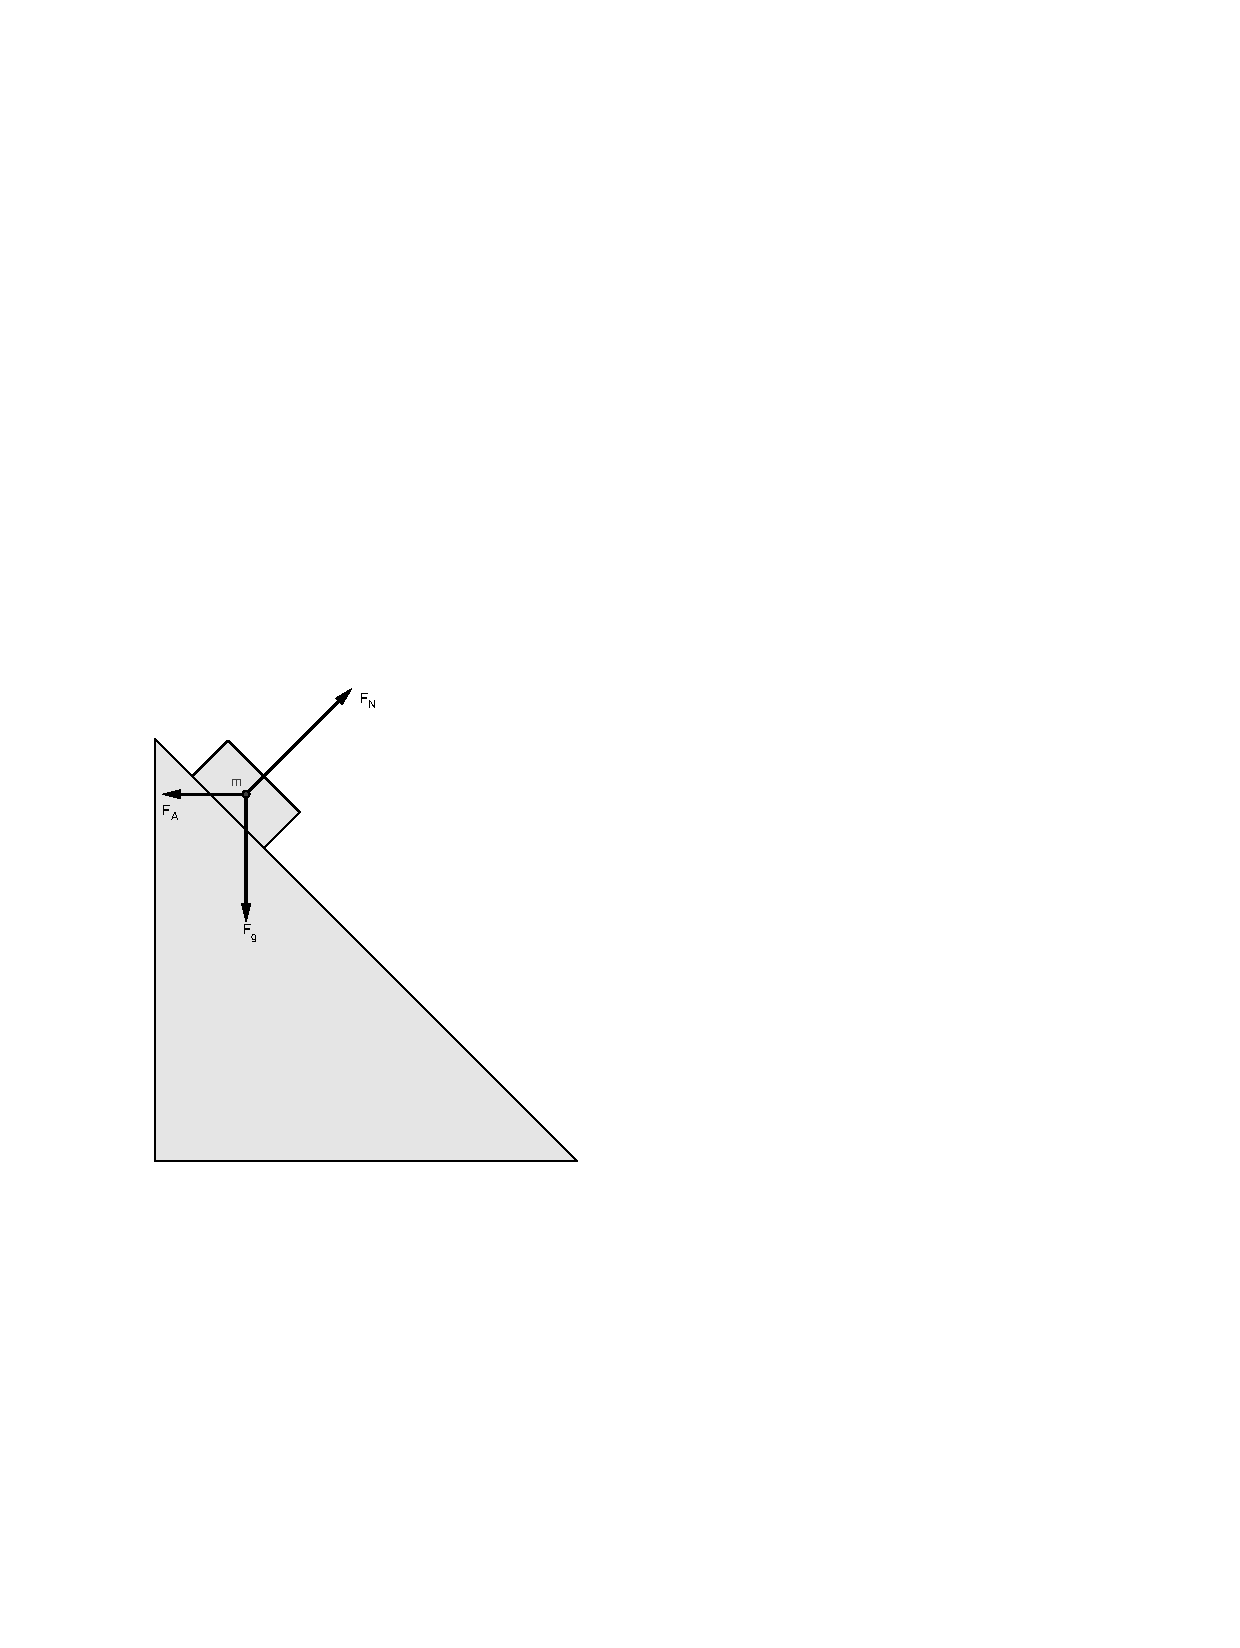
\includegraphics[width=.5\textwidth]{2009-09-25_Diagram_5}\end{center}
  Decomposing the vectors, we get the following.
  \begin{center}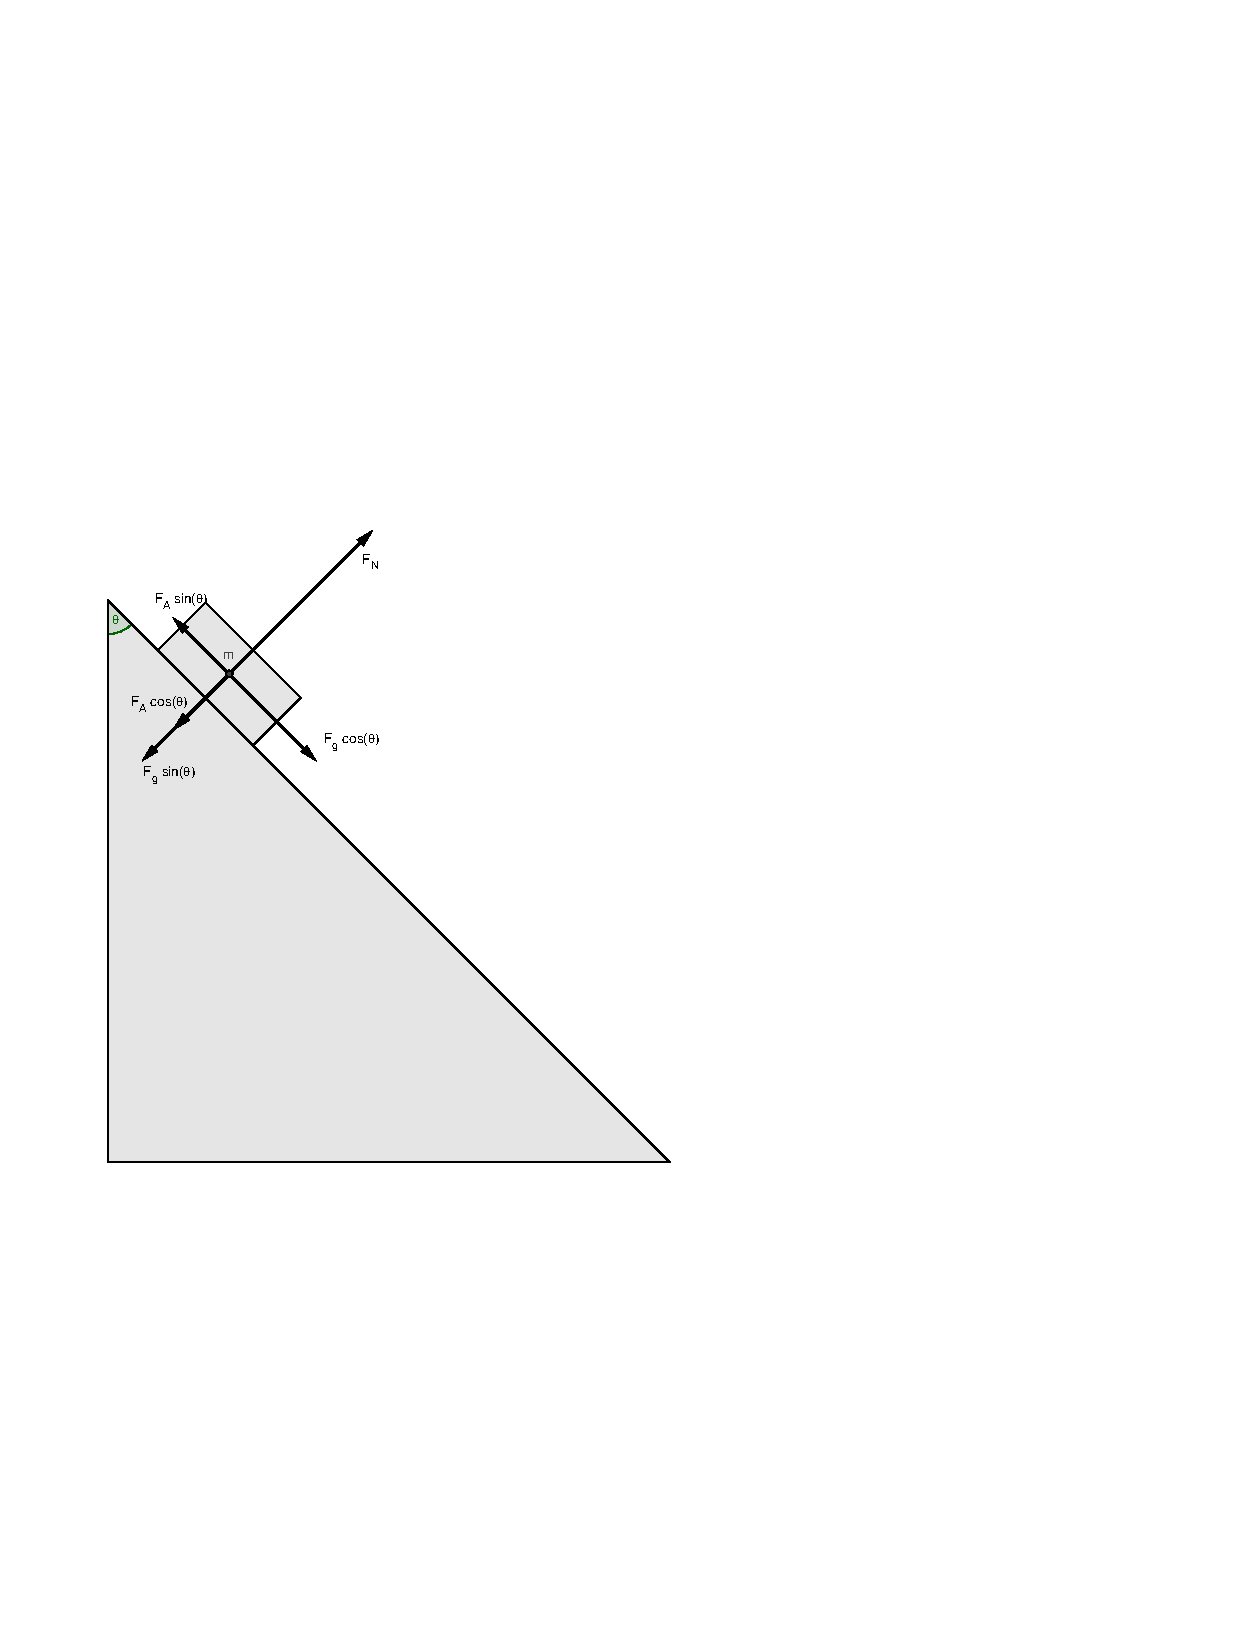
\includegraphics[width=.5\textwidth]{2009-09-25_Diagram_6}\end{center}

  Since $\sin(45^{\circ}) = \cos(45^{\circ}) = \frac{1}{\sqrt{2}}$, the magnitude of the net force is $\frac{1}{\sqrt{2}}(F_g - F_A)$ down the wedge.  Then the acceleration is $\frac{1}{\sqrt{2}}(g - A)$ down the wedge.  Transforming back to the original coordinate system, the net acceleration is $A \hat i + \frac{1}{\sqrt{2}}(g - A)\left(\frac{1}{\sqrt{2}}\hat i - \frac{1}{\sqrt{2}} \hat j\right) = \frac{1}{2}(g + A) \hat i - \frac{1}{2}(g - A)\hat j$.

  %The normal force of the wedge on the block, $F_n$, opposes the
\section{Problem \thesection: K\&K 2.22}
\subsection{Problem}
  Suppose a rope of mass $m$ hangs between two trees. The ends of the rope are at the same height and they make an angle $\theta$ with the trees.
  \begin{center}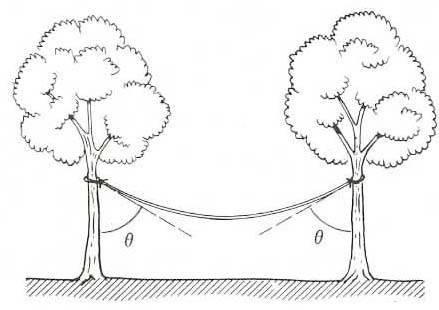
\includegraphics[width=0.35\textwidth]{ps02_5}\end{center}
  \begin{enumerate}[a)]
    \item What is the tension at the ends of the rope where it is connected to the trees?
    \item What is the tension in the rope at a point midway between the trees?
  \end{enumerate}
\subsection{Solution}
  \begin{enumerate}[a)]
    \item The magnitude of tension at the end of the rope, $T$, is such that $2T\cos\theta = mg$, so $T = \frac{mg}{2\cos\theta}$.
    \item Since there are no external horizontal forces on the rope, and no portion of the rope is accelerating, the horizontal component of tension must be constant throughout the rope.  Then $T = \frac{mg}{2}\tan\theta$. %The rope is divided into segments, as follows: \begin{center}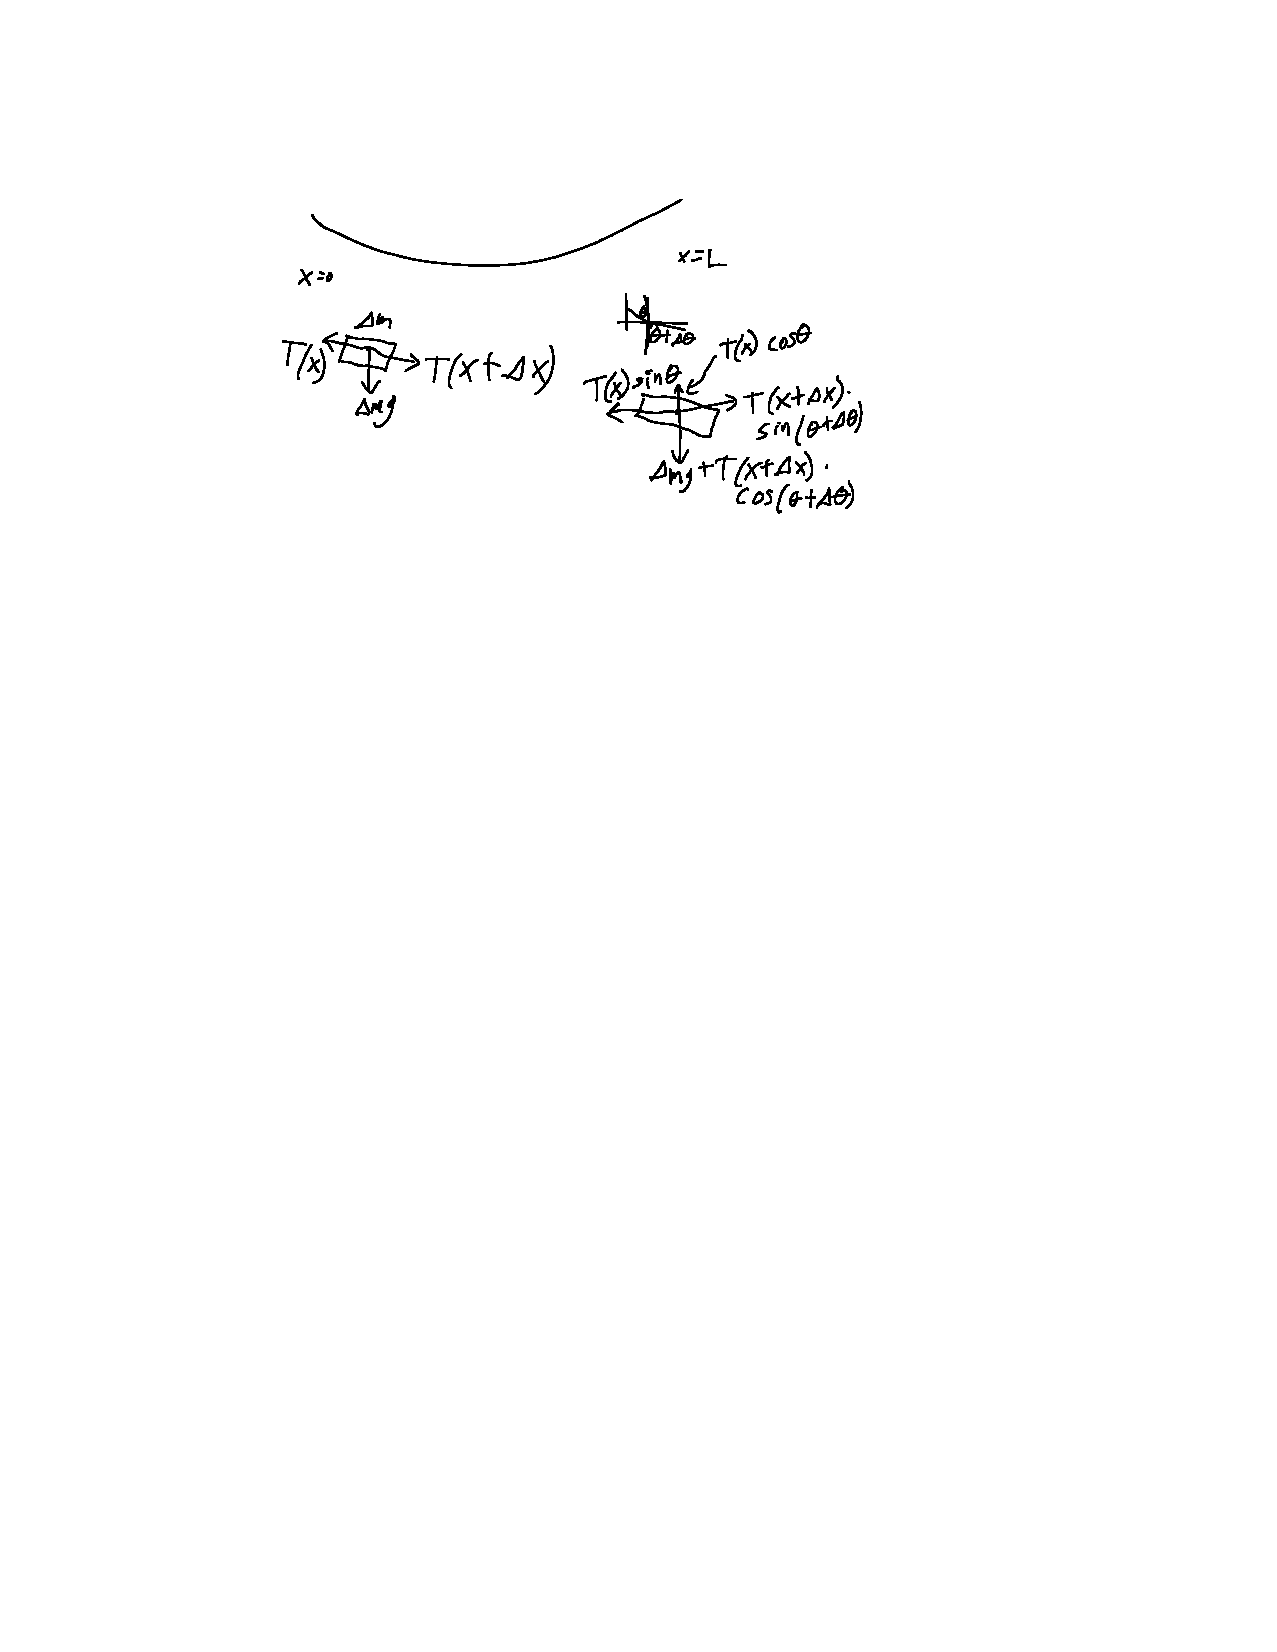
\includegraphics[width=.5\textwidth]{2009-09-25_Diagram_11_old}\end{center}  %Then \begin{align*}
  %    T(x)\cos(\theta(x)) & = \Delta m g+ T(x + \Delta x)\cos(\theta(x)+\Delta\theta) \\
  %    T(x)\sin(\theta(x)) & = T(x+\Delta x)\sin(\theta(x)+\Delta\theta) \\
  %    \\
  %    T(x + \Delta x) & = \frac{T(x)\cos(\theta(x)) - \Delta m g}{\cos(\theta(x)+\Delta\theta)} \\
  %    T(x + \Delta x) & = \frac{T(x)\sin(\theta(x))}{\sin(\theta(x)+\Delta\theta)} \\
  %    \\
  %    T(x) & = \frac{\Delta m g+ T(x + \Delta x)\cos(\theta(x)+\Delta\theta)}{\cos(\theta(x))} \\
  %    T(x) & = \frac{T(x+\Delta x)\sin(\theta(x)+\Delta\theta)}{\sin(\theta(x))} \\
  %    \\
  %    T(x+\Delta x) - T(x) & = T(x+\Delta x)\left( 1 - \frac{\sin(\theta(x)+\Delta\theta)}{\sin(\theta(x))}\right) \\
  %      & = T(x+\Delta x)\left( -\frac{\sin(\theta(x)+\Delta\theta) - \sin(\theta(x))}{\sin(\theta(x))}\right) \\
  %    \\
  %    \lim_{\Delta x \longrightarrow 0} \frac{T(x+\Delta x) - T(x)}{\Delta x} & = -\lim_{\Delta x\longrightarrow 0}\frac{T(x+\Delta x)}{\sin(\theta(x))}\lim_{\Delta x\longrightarrow 0} \frac{\sin(\theta(x)+\Delta\theta) - \sin(\theta(x))}{\Delta x} \\
  %    \\
  %    \frac{d}{d x} T(x) & = -\frac{T(x)}{\sin(\theta(x))}\cdot \frac{d}{d x} \sin(\theta(x)) \\
  %     & = -\frac{T(x)}{\sin(\theta(x))}\cos(\theta(x))\frac{d}{d x}\theta(x) \\
  %  \end{align*} FIX %Since the rope is not accelerating, the tension is uniform throughout, so $T = \frac{mg}{2\cos\theta}$.
  \end{enumerate}
\end{document}
